\documentclass[a4paper,12pt]{article}   % papír A4, písmo 12 bodu
\usepackage[utf8x]{inputenc}            %kodovaní UTF-8
\usepackage{ucs}                        %kodovani unicode
\usepackage[czech]{babel}               %podpora cestiny
\usepackage[T1]{fontenc}                %pouzij variantu pisma T1 (hacky, carky)
\usepackage[left=2.5cm,right=1.5cm,top=2.5cm,bottom=2.5cm]{geometry} %okraje stranky
\usepackage{amsmath,amsfonts,amssymb}   %podpora matematiky
\usepackage{gensymb,marvosym}           %symboly celsius (\celsius) apod.
%\usepackage{mathptmx}                   %font Times New Roman s~podporou matematiky
\usepackage{times}                      %font Times New Roman (matematika pismem Computer Modern) 
\usepackage{parskip}                    %mezera mezi odstavci
%\usepackage[document]{ragged2e}         %text zarovany vlevo
\usepackage[none]{hyphenat} \sloppy     %slova nedelit a~nepretekat
\usepackage{titlesec}
\setcounter{secnumdepth}{4}
\clubpenalty 10000                      %kontrolovat sirotky
\widowpenalty 10000                     %kontrolovat vdovy
\usepackage{setspace} \onehalfspacing   %podpora pro zmenu radkovani + radkovani 1,5
\usepackage{enumerate}                  %podpora pro zmenu cislovani
\usepackage{fancyhdr}                   %vlastni zahlavi a~zapati
\usepackage{graphicx}                   %podpora grafiky
\graphicspath{{materialy/}}                   %vychozi adresar s~obrazky
\usepackage{caption}                    %popisky
\usepackage{subcaption}                 %podpopisky
\usepackage{siunitx}
\usepackage{MnSymbol,wasysym}
\usepackage[shortlabels]{enumitem}
\usepackage{amsmath}
\usepackage{lastpage}                   %zjištění poslední stránky \pageref{LastPage}
\usepackage{float}                      
\usepackage{url}
\usepackage[unicode]{hyperref}          %klikaci odkazy v~textu
\usepackage{mhchem}
\usepackage{multirow}

\usepackage{halloweenmath}


\titleclass{\subsubsubsection}{straight}[\subsection]
\newcounter{subsubsubsection}[subsubsection]
\renewcommand\thesubsubsubsection{\thesubsubsection.\arabic{subsubsubsection}}
\renewcommand\theparagraph{\thesubsubsubsection.\arabic{paragraph}} % optional, useful if paragraphs are to be numbered


%------------------------ čtvrtá a~pátá úroveň nadpisu ---------------------------

\titleformat{\subsubsubsection}
  {\normalfont\normalsize\bfseries}{\thesubsubsubsection}{1em}{}
\titlespacing*{\subsubsubsection}
{0pt}{3.25ex plus 1ex minus .2ex}{1.5ex plus .2ex}

\makeatletter

\renewcommand\paragraph{\@startsection{paragraph}{5}{\z@}%
  {3.25ex \@plus1ex \@minus.2ex}%
  {-1em}%
  {\normalfont\normalsize\bfseries}}
\renewcommand\subparagraph{\@startsection{subparagraph}{6}{\parindent}%
  {3.25ex \@plus1ex \@minus .2ex}%
  {-1em}%
  {\normalfont\normalsize\bfseries}}
\def\toclevel@subsubsubsection{4}
\def\toclevel@paragraph{5}
\def\toclevel@paragraph{6}
\def\l@subsubsubsection{\@dottedtocline{4}{7em}{4em}}
\def\l@paragraph{\@dottedtocline{5}{10em}{5em}}
\def\l@subparagraph{\@dottedtocline{6}{14em}{6em}}
\makeatother

\setcounter{secnumdepth}{4}
\setcounter{tocdepth}{4}


\setlist[enumerate]{itemsep=0mm}
%_____________________________|___________________________|_____________________________%
%                             |                           |                             %
%-----------------------------| ZDE VYPLNIT UDAJE O PRACI |-----------------------------%
%_____________________________|___________________________|_____________________________%
%                             

\newcommand{\nazev}{ČÍSLICOVÝ MĚŘIČ IMPEDANCÍ A~ADMITANCÍ}                                                        %
\newcommand{\jmeno}{Jakub Dvořák}                                                     %
\newcommand{\datum}{\today}                                                              %
%---------------------------------------------------------------------------------------%


%-----------------------------| POUŽITÁ MAKRA |-----------------------------%

%\newcommand{\zkratka}{ve výsledku se mi napíše tenhle text}
%\newcommand{}{}
%\newcommand{}{}
%\newcommand{}{}
\newcommand{\tsub}[1]{$_\textrm{#1}$}
\newcommand{\texp}[1]{$^\textrm{#1}$}
\newcommand{\tohm}{$\Omega$}
\newcommand{\tmu}{$\mu$}


%_______________________________________________________________________________________%
%_______________________________________________________________________________________%


%----------------------------------- KONEC PREAMBULE -----------------------------------%






%-------------------------------------- DOKUMENT --------------------------------------%
%______________________________________________________________________________________%
\begin{document} %%%%%%%%%%%%%%%%%%%%%%%%%%%%%%%%%%%%%%%%%%%%%%%%%%%%%%%%%%%%%%%%%%%%%%%

\setcounter{page}{0} %cislo strany
\pagestyle{empty} %stranku necislovat

%prostredi pro grafy a~schemata \begin{graf} \begin{schema}
\newfloat{schema}{htbp}{schema}\floatname{schema}{Schéma}
\newfloat{graf}{htbp}{graf}\floatname{graf}{Graf}

\begin{titlepage}
    \begin{center}
        \vspace*{1cm}
            
        \Huge
        \textbf{\nazev}
            
        \vspace{0.5cm}
        \LARGE
            
        \vspace{1.5cm}
            
        \textbf{\jmeno}
            
        \vfill
            
        \vspace{0.8cm}
            
        \Large
            
        \datum\\
        \vspace*{.5cm}
        
\includegraphics[width=.4\textwidth]{logo-cvut-fee.png}\\
    \end{center}
\end{titlepage}

% --- definice zapati a~cislovani ---
\newpage 
\pagestyle{fancy}                                       %vlastni zahlavi/zapati
\renewcommand{\headrulewidth}{0pt}                      %bez linky v~zahlavi
\renewcommand{\footrulewidth}{.5pt}                    %linka v~zapati - optional
\lhead{}       \chead{} \rhead{\nazev}                        %pole zahlavi (prazdna)
\lfoot{\jmeno} \cfoot{} \rfoot{\thepage}   %pole zapati


%------------------------------------ VLASTNÍ TEXT ------------------------------------%



\section{Úkol měření}
\label{chap:ukol}
\begin{figure}[h!]
  \centering
  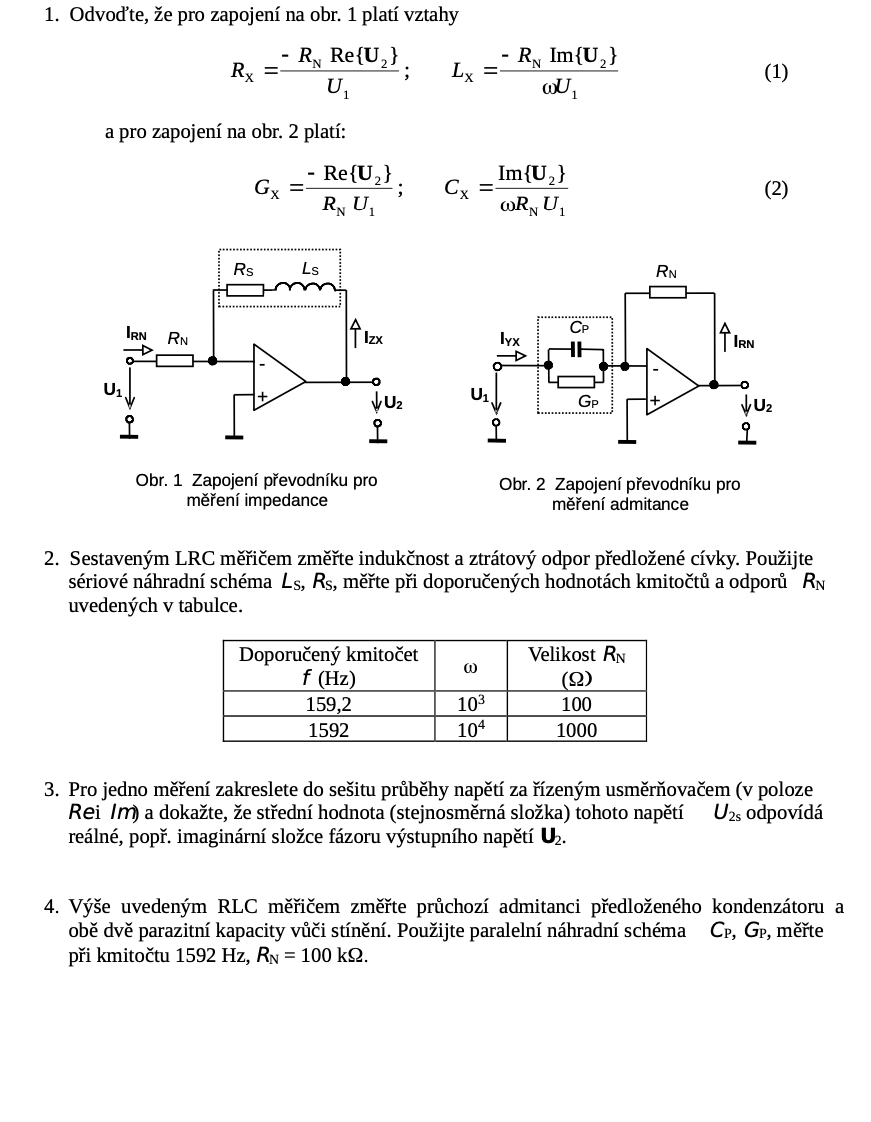
\includegraphics[width=\textwidth]{zadani.png}
\end{figure}


\section{Schéma zapojení}
\label{chap:schema_zapojeni}
\begin{figure}[h!]
  \centering
  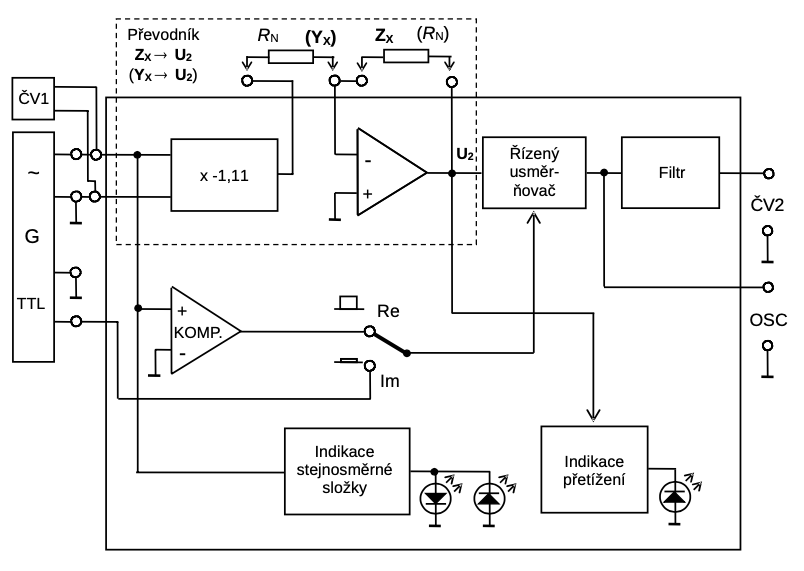
\includegraphics[width=.5\textwidth]{schema.png}
  \caption{Schéma zapojení přípravku pro měření impedancí a~admitancí}
  \label{fig:schema}
\end{figure}


\section{Seznam použitých přístrojů}
\label{chap:seznam_pristroju}
\begin{table}[h!]
  \centering
  \begin{tabular}{ll}
    G &- generátor napětí\\
    ČV1,2 &- číslicové voltmetry, AC a DC\\
    RN &-odporová dekáda\\\hline
    \multicolumn{2}{l}{Napájecí zdroj $\pm$ 15~V}\\
  \end{tabular}
\end{table}


\section{Teoretický úvod}
\label{chap:teoreticky_uvod}
Pro měření reálné a imaginární složky výstupního napětí $\hat{U_\text{2}}$ využíváme řízený usměrňovač. Jako referenční napětí pro řízení přepínače použijeme při měření reálné složky napájecí napětí $\hat{U_\text{1}}$ volené komparátorem. Pro měření imaginární složky použijeme pro řízení usměrňovače TTL výstup z generátoru., které je posunuto o $\frac{\pi}{4} = 90~\degree$. 

\subsubsection{Odvození vztahů}
\begin{equation}
  \begin{split}
    \hat{I}_\text{RN} &= -\hat{I}_\text{ZX}\\
    \frac{\hat{U}_\text{1}}{R_\text{N}} &= -\frac{\hat{U}_\text{2}}{Z_\text{X}}\\
    \hat{Z}_\text{X} &= -\frac{R_\text{N}\hat{U}_\text{N}}{U_\text{1}}\\
    L_\text{X} &= -\frac{R_\text{N}\text{Im}\{\hat{U}_\text{2}\}}{\omega U_\text{1}}\\
  \end{split}
\end{equation}
\begin{equation}
  \begin{split}
    \hat{I}_\text{YX} &= -\hat{I}_\text{RN}\\
    &\dots\\
    C_\text{x} &= -\frac{Im\{\hat{U}_\text{2}\}}{\omega R_\text{N}{U}_\text{1}}
  \end{split}
\end{equation}

\section{Naměřené hodnoty}
\label{chap:namerene_hodnoty}
Naměřené hodnoty jsou v tabulce níže

\begin{table}[h!]
  \centering
  \begin{tabular}{|c|c|c|c|c||c|}
    \hline
    \multicolumn{6}{|c|}{Cívka}       \\ \hline
    f[Hz]     & R[\tohm]    & U[V]    & Re[V]   & Im[V] & L[H]  \\ \hline
    159,2 & 100  & 1,03    & 0,02 & 0,66 & \textbf{0,66} \\ \hline\hline
    \multicolumn{6}{|c|}{Kondenzátor} \\ \hline
    f[Hz]     & R[\tohm]    & U[V]    & Re[mV]   & Im[V] & C[nF]  \\ \hline
    159,2 & 1000 & 1,02 & 26,6 & 1,01 & \textbf{1,009}\\ \hline
  \end{tabular}
\end{table}



\section{Zpracování naměřených hodnot}
\label{chap:zpracovani_hodnot}
\begin{figure}[h!]
  \centering
  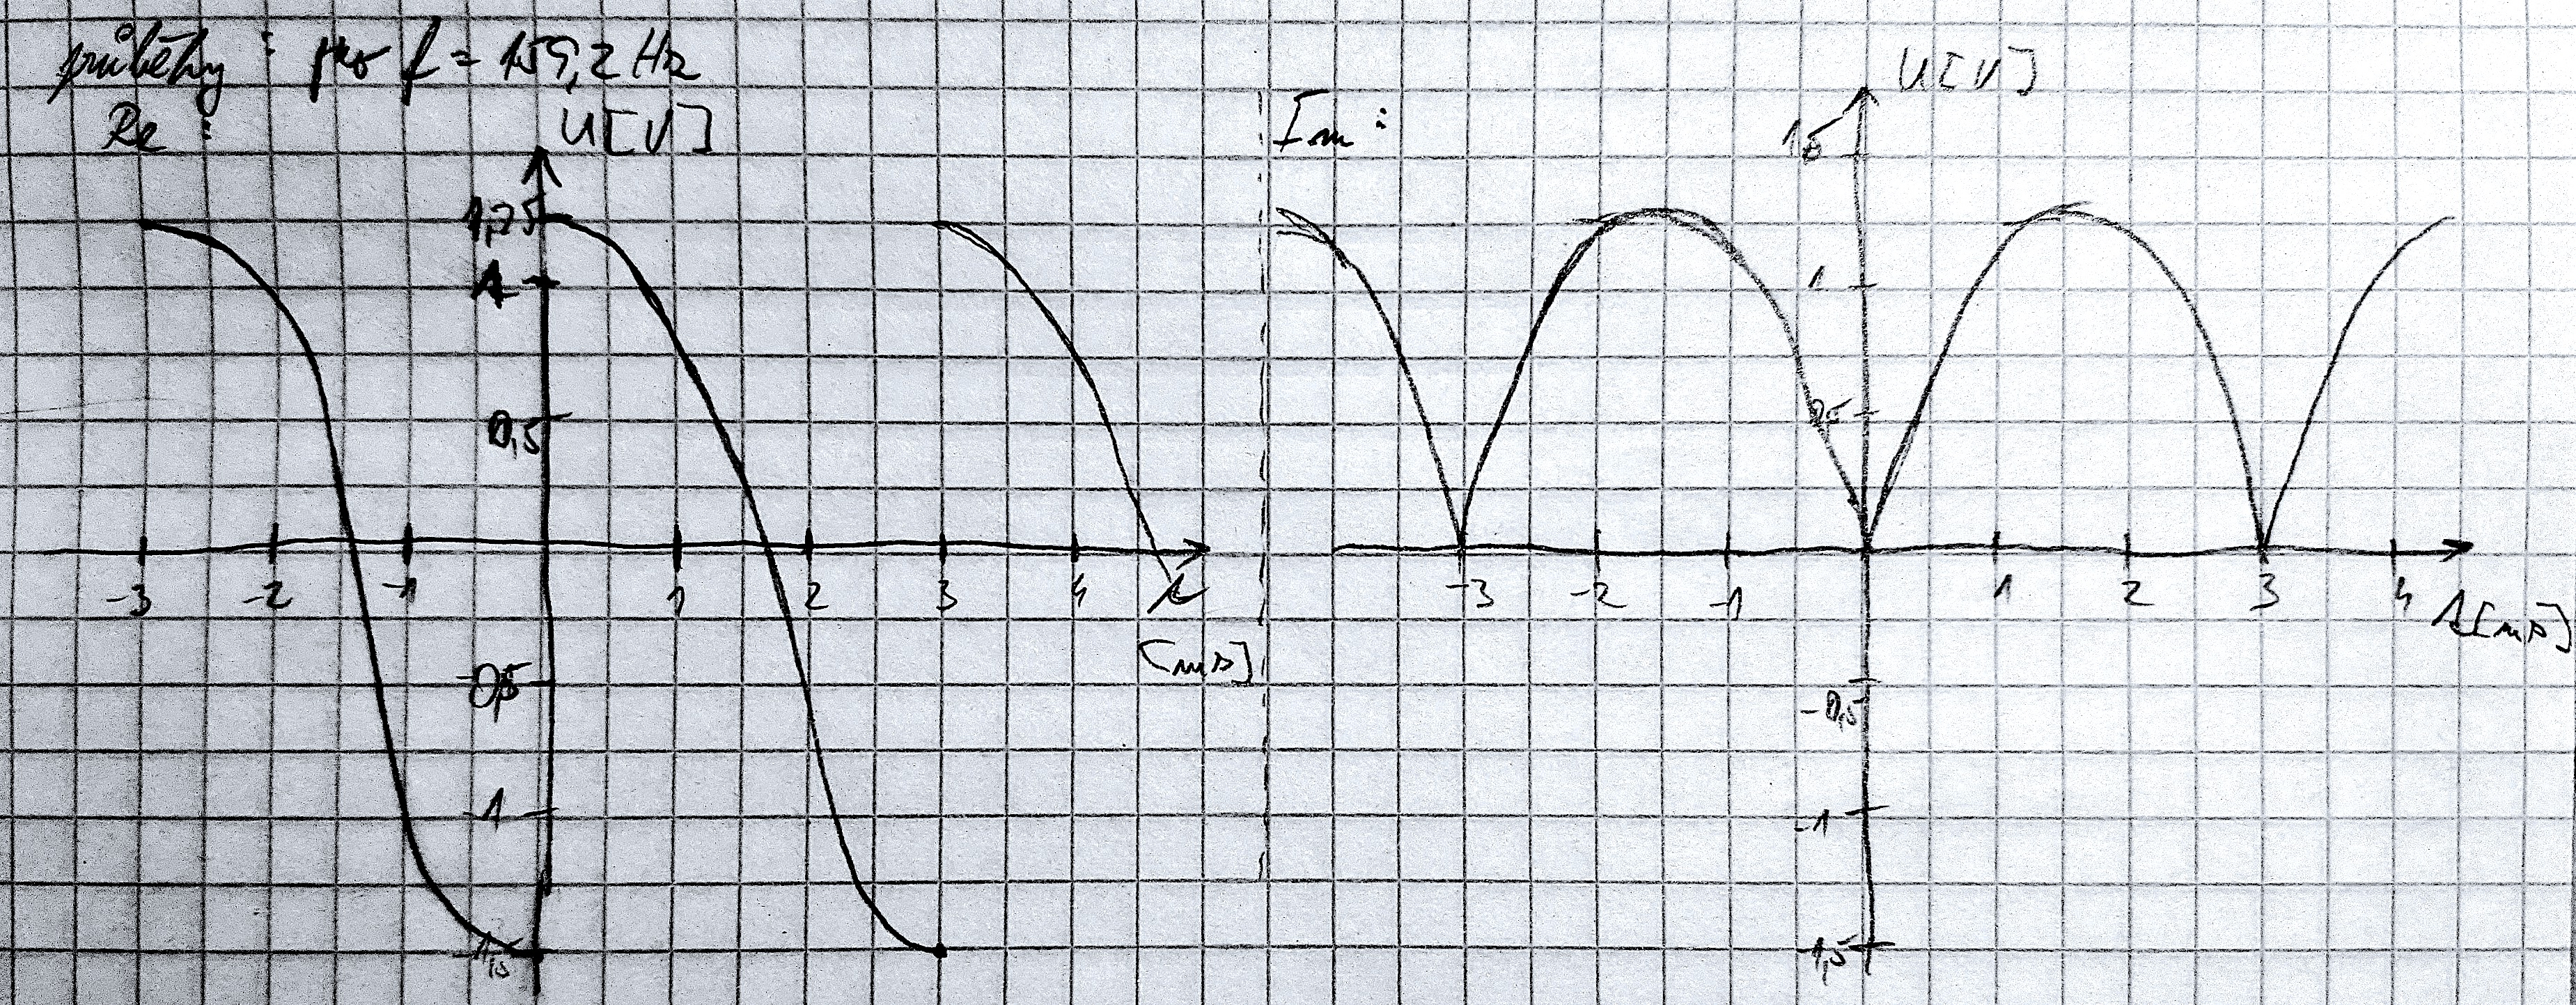
\includegraphics[width=\textwidth]{prubeh.jpg}
  \caption{Nakreslené průběhy napětí na čase}
\end{figure}

\subsubsection{Terminování kondenzátoru}
\begin{equation}
  \begin{split}
    \text{Im}\{\hat{U}_\text{2}\} = 1,11~\text{V}\\
    \text{Im}\{\hat{U}_\text{2}\} = 1,26~\text{V}\\
    C_{20} = -\frac{\text{Im}\{\hat{U}_\text{2}\}}{\omega R_\text{N}U_\text{1}}-C_\text{12} = \underline{100~\text{nF}}\\
    C_{10} = -\frac{\text{Im}\{\hat{U}_\text{2}\}}{\omega R_\text{N}U_\text{1}}-C_\text{12} = \underline{250~\text{nF}}\\
  \end{split}
\end{equation}


\section{Závěrečné vyhodnocení}
\label{chap:zaver}
Naměřili jsme indukčnosti cívky a kapacitu kondenzátoru. U Kondenzátoru jsme také správně určili jeho parazitní kapacity vůči stínění, které se mezi sebou lišily a jejich hodnota byla přibližně 10~\% z kapacity kondenzátoru. Také jsme ověřili průběhy reálné a imaginární složky proudu resp. napětí.


%--- LITERATURA a~ZDROJE (povinne) ---
\clearpage
\renewcommand{\refname}{Seznam použité literatury a~zdrojů informací} 
%\section*{Seznam použité literatury a~zdrojů informací}
\phantomsection %pridej odkaz do PDF zalozek
\addcontentsline{toc}{section}{Seznam použité literatury a~zdrojů informací}

\begin{thebibliography}{99}

%----------------------------------------------------
\subsection*{Seznam použitých internetových zdrojů}
    \bibitem{navod} Návod k~laboratorní úloze
    
\end{thebibliography}

\end{document}